\documentclass[12pt,a4paper]{article} 

\usepackage[russian]{babel}
\usepackage[T2A]{fontenc} 
\usepackage[utf8]{inputenc} 
\usepackage{graphicx}
\usepackage{amsmath}
\usepackage{amssymb}
\usepackage{amsfonts}
\usepackage{geometry}

\geometry{a4paper, total = {170mm, 257mm}, left = 20mm, top = 20mm}
\frenchspacing 

\renewcommand{\baselinestretch}{1.3}

% counter
\newcounter{problem}
\renewcommand{\theproblem}{\arabic{problem}.}
\newcommand{\problem}{\refstepcounter{problem}\textbf{Задача~\theproblem~}}

% convenience commands
\newcommand{\boldVec}[1]{\vec{\mathbf #1}}
\newcommand{\vectorProduct}[2]{\boldVec #1 \times \boldVec #2}
\newcommand{\scalarProduct}[2]{(\boldVec #1, \boldVec #2)}

\begin{document}
    \begin{center}
        {\textbf 
            {\Large
                Дифференциальная геометрия
                \\
                Домашнее задание №1
                \\
                <<Кривые и поверхности в пространстве>>
                \\
                ФН2-42Б, 2 курс, 4 семестр
                \\
                Арсений Токарев, Вариант 2-23
                \\
            }
        }
    \end{center}

    \section*{Дано: }

    \hspace{5mm} Поверхность задана параметрически уравнениями $ S \colon \boldVec r = \boldVec r(u, v), \  u, v \in \mathbb{R} $.

    Уравнение поверхности: 
    \[ \boldVec r(u, v) = \{ \cosh u \cos v,\ 5 \sinh u,\ \cosh u \sin v \}. \]

    Вид кривой на поверхности и координаты точек: 
    \[ \gamma \colon u = v;\ P_1(1, 0, 0);\ P_2(-\cosh \pi, 5 \sinh \pi, 0). \]

    \section*{Задачи: }


    \hspace{7mm}\problem Найти особые точки параметризированной поверхности. Составить уравнение касательной к поверхности в точках $ P_1 $ и $ P_2 $.
    
    \bigskip

    Для того, чтобы вывести уравнение касательной плоскости к поверхности в точке, необходимо найти вектор к поверхности в данной точке. Сначала нужно взять частные производные $ \frac{\partial \boldVec r}{\partial u} = \boldVec r_u $ и $ \frac{\partial \boldVec r}{\partial v} = \boldVec r_v $: 
    \[
        \boldVec r_u = 
            \begin{pmatrix}
                \sinh u \cos v
                \\
                5\cosh u
                \\
                \sinh u \sin v
            \end{pmatrix}\! ; \  
        \boldVec r_v = 
            \begin{pmatrix}
                -\cosh u \sin v
                \\
                0
                \\
                \cosh u \cos v
            \end{pmatrix}\! ,
    \]

    \noindent затем векторно их перемножить:
    \[
        \vectorProduct{r _u}{r_v} = 
            \begin{vmatrix}
                i && j && k
                \\
                \sinh u \cos v && 5\cosh u && \sinh u \sin v
                \\
                -\cosh u \sin v && 0 && \cosh u \cos v
            \end{vmatrix}
        =
    \]

    \noindent $ = \boldVec i\,(5 \cosh^2 u \cos u ) + \boldVec j\,(\sinh u \cosh u \cos^2 - \sinh u \cosh u \sin^2 v) + \boldVec k\,(5 \cosh^2 u \sin v) $
    \[
       \vectorProduct{r_u}{r_v} =
        \begin{pmatrix}
            5 \cosh^2 u \cos v
            \\
            -\sinh u \cosh u
            \\
            5 \cosh^2 u \sin v
        \end{pmatrix}\! .
    \]

    Сразу можно заметить, что $ \boldVec r_u \times \boldVec r_v \ne \vec{\textbf 0}$ ни при каких значениях $ u \ \text{или} \ v $. Это означает, что все точки поверхности -- регулярные.

    Посчитаем норму векторного призведения $ | \boldVec r_u \times \boldVec r_v | $: 
    \[
        | \boldVec r_u \times \boldVec r_v | = \sqrt{25 \cosh^4 u + \sinh^2 y \cosh^2 u} = \cosh u \sqrt { 25 \cosh^2 u + \sinh^2 u }\, . 
    \]

    Таким образом, вектор нормали $ \vec{\textbf n} $ имеет следующий вид: 
    \[
        \vec{\textbf n} = \frac{\boldVec r_u \times \boldVec r_v}{| \boldVec r_u \times \boldVec r_v |} = \frac{1}{\sqrt{25 \cosh^2 u + \sinh^2 u}}
        \begin{pmatrix}
            5 \cosh u \cos v
            \\
            -\sinh u
            \\
            5 \cosh u \sin v
        \end{pmatrix} \! .
    \]

    Выразим координаты точек $ P_1 $ и $ P_2 $ через $ u \ \text{и} \ v $. Для этого приравняем координаты уравнения поверхности $ \boldVec r(u, v) $ к координатам этих точек:
    \begin{table}[h]
        \centering
        \begin{tabular}{lcl}
            $
                P_1: 
                \begin{cases}
                    \cosh u \cos v = 1;
                    \\
                    5 \sinh u = 0;
                    \\
                    \cosh u \sin v = 0.
                \end{cases} 
            $ 
            & $ \Leftrightarrow $ & 
            $
                \begin{cases}
                    u_1 = 0;
                    \\
                    v_1 = 0.
                \end{cases}
            $

            \\ \\

            $
                P_2: 
                \begin{cases}
                    \cosh u \cos v = -\cosh \pi;
                    \\
                    5 \sinh u =  5 \sinh \pi;
                    \\
                    \cosh u \sin v = 0.
                \end{cases}
            $ 
            & $ \Leftrightarrow $ & 
            $
                \begin{cases}
                    u_2 = \pi;
                    \\
                    v_2 = \pi.
                \end{cases}
            $

        \end{tabular}
    \end{table}

    Теперь можно найти нормали касательных плоскостей в точках $ P_1 $ и $ P_2 $ соответсвенно. В точке $ {P_1} $ вектор единичной нормали равен:
    \[
        \vec{\textbf n}|_{P_1} =
        \begin{pmatrix}
            1 
            \\ 
            0 
            \\ 
            0  
        \end{pmatrix}\! ,
    \]

    \noindent тогда касательная плоскость имеет вид: 
    \[
        T|_{P_1}: x - 1 = 0.
    \]


    В точке $ {P_2} $ вектор единичной нормали равен:
    \[
        \vec{\textbf n}|_{P_2} = \frac{1}{\sqrt{25 \cosh^2 \pi + \sinh^2 \pi}}
        \begin{pmatrix}
            -5 \cosh \pi
            \\
            -\sinh \pi
            \\
            0
        \end{pmatrix}\! , 
    \]

    \noindent и касательная плоскость имеет вид: 
    \[
        T|_{P_2}: 5 \cosh \pi \cdot x + \sinh \pi \cdot y + 5 = 0.
    \]

    \bigskip

    \begin{flushright}
        \begin{tabular}{rl}
            \textbf{Ответ:} & Особых точек нет;

            \\

                            & $ T|_{P_1}: x - 1 = 0 $;

            \\

                            & $ T|_{P_2}: 5 \cosh \pi \cdot x + \sinh \pi \cdot y + 5 = 0 $.
        \end{tabular}
    \end{flushright}


    \problem Исследовать зависимость вида поверхности от области изменения параметров $ (u, v) $. Составить уравнения координатных линий. Построить поверхность и координатную сеть на ней (с использованием системы компьютерной алгебры Wolfram Mathematica)

    \bigskip
    
    Уравнение поверхности, выраженное через $ x, y, z $: 
    \[
        \begin{cases}
            x = \cosh u \cos v;
            \\
            y = 5 \sinh u;
            \\
            z = \cosh u \sin v;
        \end{cases} 
        \Leftrightarrow \ 
        x^2 + z^2 - \frac{y^2}{25} = 1, 
    \]

    \noindent значит, данная поверхность -- однополостный гиперболоид с осью вдоль $ OY $ (рис. \ref{fig:hyp}).

    \begin{figure}[!h]
        \centering
        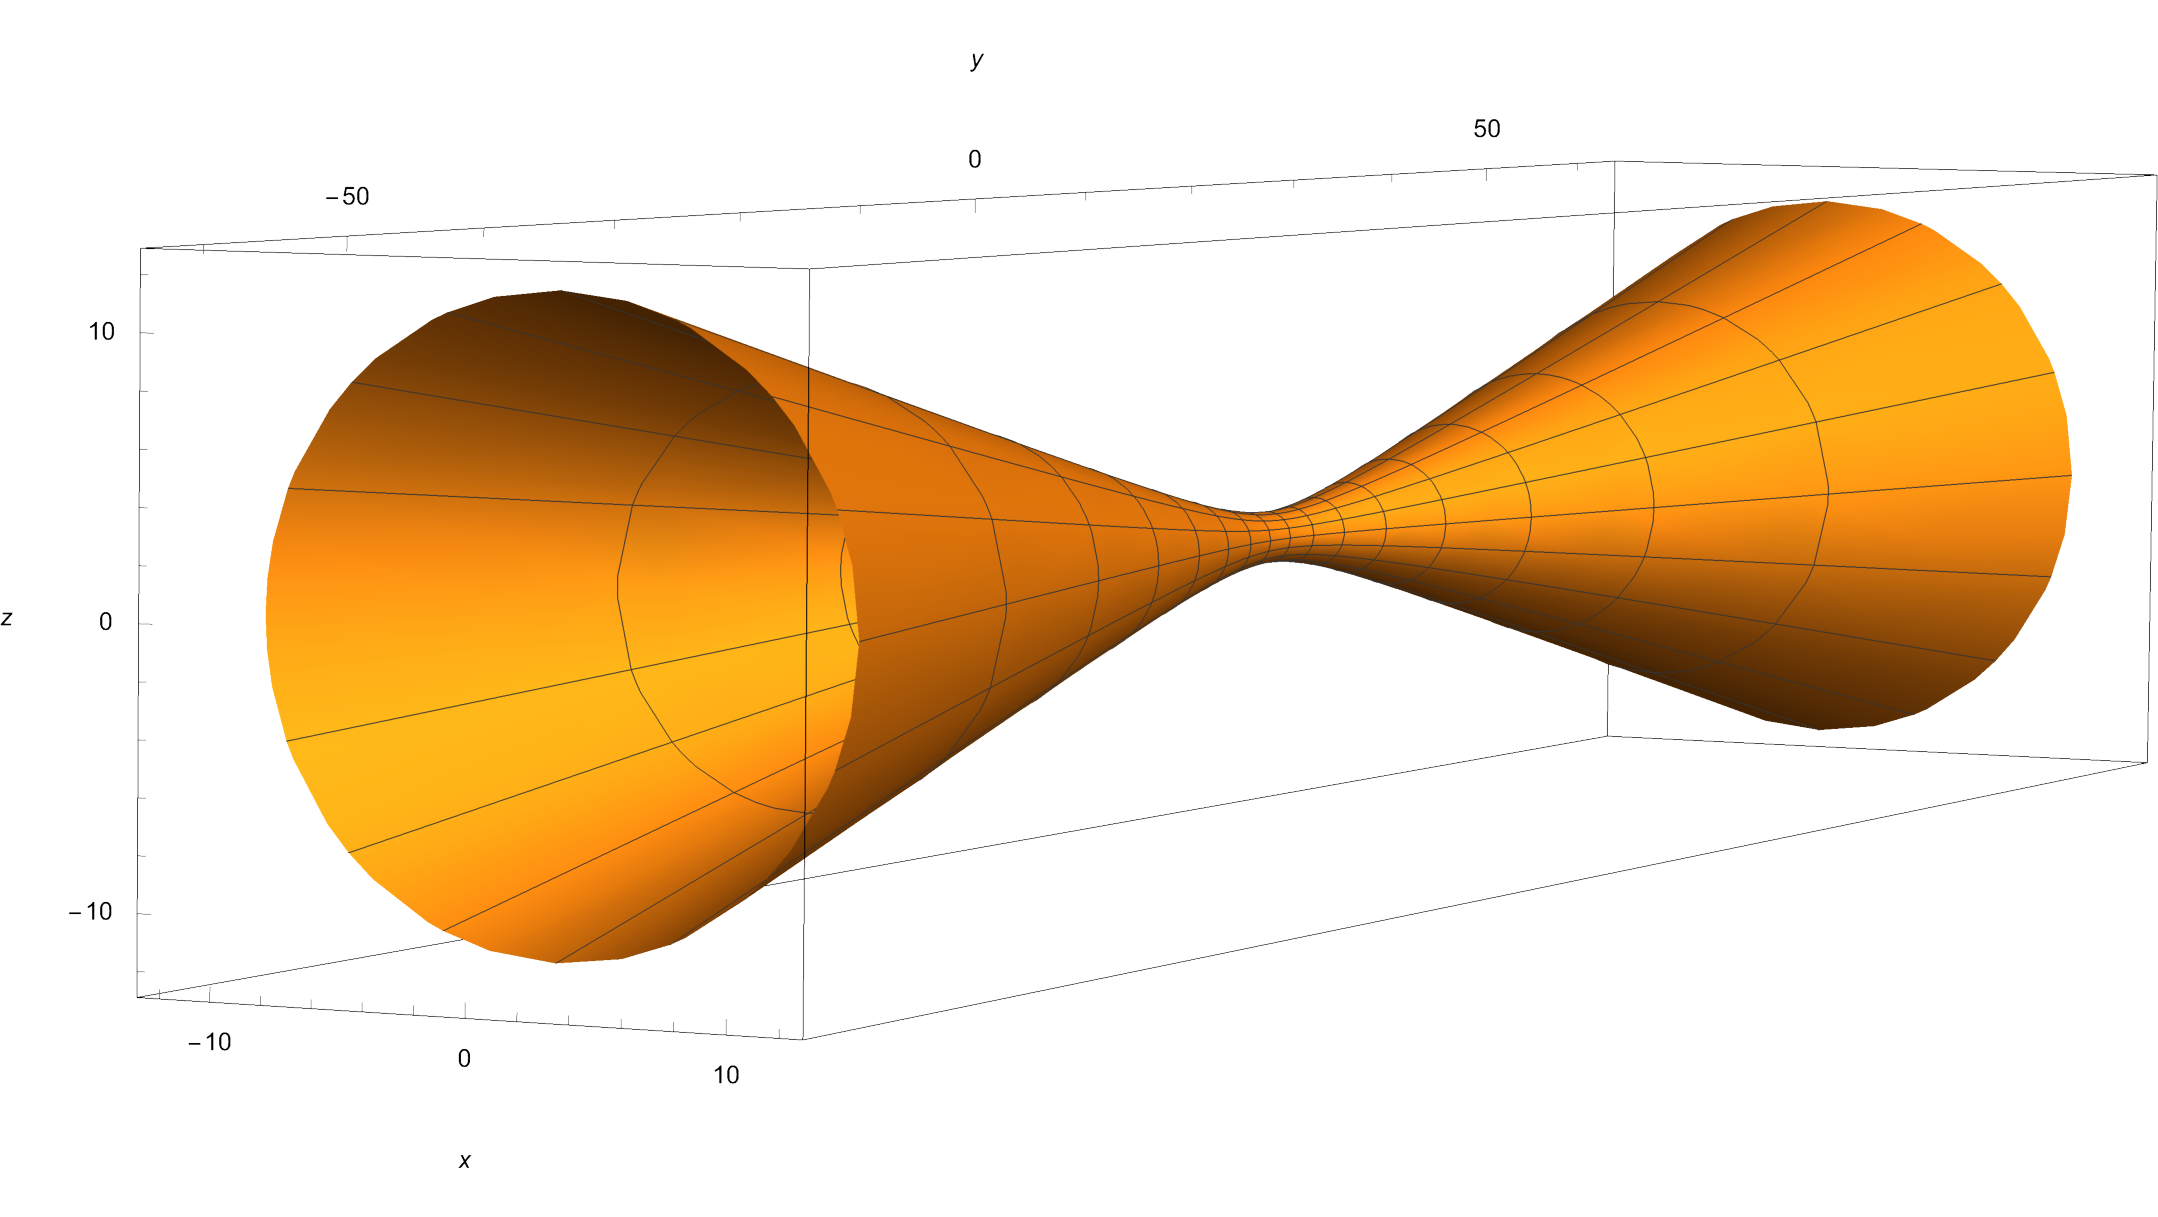
\includegraphics[width=0.8\textwidth]{Hyp.pdf}
        \caption{Однополостный гиперболоид}
        \label{fig:hyp}
    \end{figure}

    Рассмотрим координатные линии данной поверхности. При $ u_0 = const $ получаем:
    \[
        x^2 + z^2 = const,\, const = R = \sqrt{1 + \frac{y^2}{25}} = \cosh u_0,
    \]

    \noindent то есть уравнения окружностей с радиусами $R = \cosh u_0$. А при $v_0 = const$ получаем се\-мейство гипербол.

    \begin{flushright}
        \begin{tabular}{rl}
            \textbf{Ответ:} & Однополостный гиперболоид;

            \\

                            & $ (u_0, v) $ -- окружности;

            \\

                            & $ (u, v_0) $ -- гиперболы.
        \end{tabular}
    \end{flushright}

    \pagebreak

    \problem Вычислить первую квадратичную форму поверхности. Вычислить угол между кривыми $ l_1 \colon u = v^2 $ и $ l_2 \colon u = v $ в точке их пересечения.

    \bigskip

    Вычислим коэффициенты первой квадратичной формы:
    \[
        \begin{tabular}{l}
            $ E(u,v) = \scalarProduct{r_u}{r_u} = \sinh^2 u + 25 \cosh^2 u $,
            \\ \\
            $ M(u,v) = \scalarProduct{r_u}{r_v} = 0 $,
            \\ \\
            $ G(u,v) = \scalarProduct{r_v}{r_v} = \cosh^2 u $,
        \end{tabular}
    \]
    
    \noindent значит, матрица первой квадратичной формы имеет вид: 
    \[
       \mathbb{G}(u, v) = 
       \begin{pmatrix}
           \sinh^2 u + 25 \cosh^2 u & 0
           \\
           0                        & \cosh^2 u
       \end{pmatrix}\! .
    \]

    Угол между кривыми -- это угол между векторами их скоростей в точке их пересечения. Его можно вычислить по следующей формуле:
    \[
        \cos \alpha = \frac {
            (\boldVec \xi_1)^T \cdot \mathbb{G} \cdot \boldVec \xi_2
        } {
            \sqrt{(\boldVec \xi_1)^T \cdot \mathbb{G} \cdot \boldVec \xi_1} \cdot \sqrt{(\boldVec \xi_1)^T \cdot \mathbb{G} \cdot \boldVec \xi_1}
        }
    \]
    
    Для нахождения точек пересечения и для вычисления векторов скоростей параметризуем кривые $ l_1 $ и $ l_2 $:
    \begin{table}[h]
        \centering
        \begin{tabular}{lcl}
            $
                l_1: u = v^2
            $ 
            & $ \Leftrightarrow $ & 
            $
                \begin{cases}
                    u_1 = t^2;
                    \\
                    v_1 = t.
                \end{cases}
            $

            \\ \\

            $
                l_2: u = v
            $ 
            & $ \Leftrightarrow $ & 
            $
                \begin{cases}
                    u_2 = t;
                    \\
                    v_2 = t,
                \end{cases}
            $
        \end{tabular}
    \end{table}
    
    \noindent теперь найдем их точки пересечения:
    \[
        \begin{cases}
            t^2 = t;
            \\
            t = t.
        \end{cases}
        \Leftrightarrow \ 
        \begin{cases}
            t_1 = 0;
            \\
            t_2 = 1.
        \end{cases}
    \]
    
    Далее вычислим векторы скоростей кривых $ l_1 $ и $ l_2 $ в произвольной точке t:
    \begin{table}[h]
        \centering
        \begin{tabular}{l}
            $ \boldVec \xi_1(t)  = 
                \begin{pmatrix}
                    \dot u_1
                    \\
                    \dot v_1
                \end{pmatrix}
            =
                \begin{pmatrix}
                    2t
                    \\
                    1
                \end{pmatrix}\! ,
            $ 
            \\ \\
            $ \boldVec \xi_2(t)  = 
                \begin{pmatrix}
                    \dot u_2
                    \\
                    \dot v_2
                \end{pmatrix}
            =
                \begin{pmatrix}
                    1
                    \\
                    1
                \end{pmatrix}\! .
            $ 
        \end{tabular}
    \end{table}

    \pagebreak
    
    Сначала рассмотрим случай, когда $t = t_1 = 0$, тогда:
    \begin{table}[h]
        \centering
        \begin{tabular}{l}
            $ \mathbb{G}|_{t_1} = 
                \begin{pmatrix}
                    25 & 0
                    \\
                    0  & 1
                \end{pmatrix}\! ,
            $
            \\ \\
            $ \boldVec \xi_1(t_1) = \boldVec \xi_1(0) = 
                \begin{pmatrix}
                    0
                    \\
                    1
                \end{pmatrix}\! ,
            $ 
            \\ \\
            $ \boldVec \xi_2(t_1) = \boldVec \xi_2(0) = 
                \begin{pmatrix}
                    1
                    \\
                    1
                \end{pmatrix}\! ,
            $ 
        \end{tabular}
    \end{table}

    \noindent а значит угол между кривыми в точке $ t_1 $ равен:
    \[
        \cos \alpha_1 = \frac{1}{26}
        \,\Rightarrow\,
        \alpha_1 = \arccos{\frac{1}{26}} \approx 1.34^{\circ}
    \]

    Теперь рассмотрим случай. когда $ t = t_2 = 1 $, следовательно:
    \begin{table}[h]
        \centering
        \begin{tabular}{l}
            $ \mathbb{G}|_{t_2} = 
                \begin{pmatrix}
                    \sinh^2 1 + 25 \cosh^2 1 & 0
                    \\
                    0                        & \cosh^2 1
                \end{pmatrix}\! ,
            $
            \\ \\
            $ \boldVec \xi_1(t_2) = \boldVec \xi_1(0) = 
                \begin{pmatrix}
                    2
                    \\
                    1
                \end{pmatrix}\! ,
            $ 
            \\ \\
            $ \boldVec \xi_2(t_2) = \boldVec \xi_2(0) = 
                \begin{pmatrix}
                    1
                    \\
                    1
                \end{pmatrix}\! ,
            $ 
        \end{tabular}
    \end{table}

    \noindent и угол между кривыми в точке $ t_2 $ равен:
    \[
        \cos \alpha_2 \approx \frac{124.198}{246.015 \cdot 63.2896}
        \,\Rightarrow\,
        \alpha_2 \approx 0.097^{\circ}
    \]

    \begin{flushright}
        \begin{tabular}{rl}
            \textbf{Ответ:} & $ I = (\sinh^2 u + 25 \cosh^2 u)du^2 + (\cosh^2 u) dv^2 $;

            \\

                            & $ \alpha_1 = \approx 1.34^{\circ} $;

            \\

                            & $ \alpha_2 \approx 0.097^{\circ} $.
        \end{tabular}
    \end{flushright}


    % $ E(u,v) = \scalarProduct{r_u}{r_u} = \sinh^2 u + 25 \cosh^2 u $,
    %         \\ \\
    %         $ M(u,v) = \scalarProduct{r_u}{r_v} = 0 $,
    %         \\ \\
    %         $ G(u,v) = \scalarProduct{r_v}{r_v} = \cosh^2 u $,

\end{document}